% =====================================================================
%  Khóa luận tốt nghiệp
%  Trường Đại học Công nghệ - Đại học Quốc gia Hà Nội
%
%  Đề tài: Phương pháp tạo dữ liệu kiểm thử thủ công cho đối tượng atomic trong dự án C++
%  Sinh viên: Lưu Quang Tùng - MSSV 23020150
%  Cán bộ hướng dẫn: PGS.TS. Phạm Ngọc Hùng, TS. Trần Hoàng Việt
%
%  Cách compile (BẮT BUỘC dùng LuaLaTeX hoặc XeLaTeX vì template dùng fontspec):
%      PATH="$HOME/.local/bin:$PATH" latexmk -f -lualatex -interaction=nonstopmode main.tex
%
%  Các việc cần làm:
%    1. Thông tin trên bìa nằm ở chapters/0-coverpage.tex (năm tự lấy theo \the\year)
%    2. Tài liệu tham khảo: refs.bib (entry có keywords = {vietnam} sẽ in ở mục "Tiếng Việt")
%    3. Nội dung các chương: thư mục chapters/
% =====================================================================
\documentclass[13pt,a4paper,oneside]{book} % twoside for draf

\usepackage[justification=centering]{caption}
% \usepackage{babel}
%\usepackage{times} \usepackage{graphicx}
% ---------------------------------------------------------------------
% LƯU Ý THỨ TỰ NẠP GÓI FONT:
%   mathptmx (font toán kiểu Times) BẮT BUỘC nạp TRƯỚC fontspec,
%   vì mathptmx có lệnh \def\rmdefault{ptm} -> nếu nạp sau fontspec thì nó sẽ
%   ghi đè \setmainfont và toàn bộ văn bản sẽ bị LaTeX thay bằng font Latin Modern
%   thay vì Times New Roman.
% ---------------------------------------------------------------------
\usepackage{mathptmx}   % same Time New Roman (nạp TRƯỚC fontspec - xem lưu ý trên)
\usepackage{fontspec}
\setmainfont{Times New Roman}
\usepackage{amsmath} 
\usepackage{indentfirst}

%\renewcommand{\rmdefault}{phv} % Arial \renewcommand{\sfdefault}{phv} % Arial \usepackage[fontsize=13pt]{scrextend}


\usepackage{fancyhdr}
% \usepackage[utf8]{inputenc}
\usepackage[vietnamese, english]{babel}
\usepackage{titlesec}

\usepackage{titletoc}
\usepackage{listings}
\usepackage[bookmarks=true]{hyperref}
\usepackage[left=3cm,right=2cm,top=2.5cm,bottom=3cm]{geometry}
\usepackage{graphicx}
\usepackage{hyperref}
\usepackage{tikz}
\usepackage{varwidth}
\usepackage{graphicx}
\usepackage{float}
\usepackage{color}
\usepackage{multirow}
\usepackage{booktabs}
% Gói thuật toán: dùng combo algorithm + algpseudocode (khớp với nội dung các chương).
% KHÔNG dùng algorithm2e vì nó xung đột với algpseudocode (\If, \Else, \EndIf).
\usepackage{algorithm}
\usepackage{algpseudocode}   % hỗ trợ môi trường algorithmic (\State, \If, \Require, ...) dùng trong nội dung các chương
\floatname{algorithm}{Thuật toán}
\counterwithin{algorithm}{chapter}   % đánh số thuật toán theo chương: 2.1
\usepackage{svg}
\usepackage{tabularx}
\usepackage{nomencl}
\usepackage{scrfontsizes}
\usepackage{longtable}
\usepackage{multicol}
\usepackage{enumitem}   % hỗ trợ tùy chỉnh danh sách: \begin{itemize}[leftmargin=*, itemsep=0.3em]
\usepackage[toc,page]{appendix}
\usepackage{adjustbox}
\usepackage{setspace}
% \usepackage{algorithm} \floatname{algorithm}{Thuật toán} \usepackage{algpseudocode}

\usepackage{makecell}
\usepackage{longtable}
\usepackage{multirow}
% \usepackage{algpseudocode}
\usepackage{setting/bkthesis}
\usepackage[toc]{appendix}

%\counterwithin{figure}{chapter}
\usepackage[ defernumbers, sortcites, backend=biber, bibstyle=authoryear, sorting=none, citestyle=numeric-comp
]{biblatex}
\usepackage{xpatch}
\usepackage{tikz}
\usetikzlibrary{shapes.geometric}
\usepackage{forest}   % vẽ cây dữ liệu (Data Tree) trong chương Phương pháp đề xuất
\usetikzlibrary{arrows.meta,arrows}
\titlelabel{\thetitle. }

% \usepackage{csquotes}
% \DeclareQuoteStyle{vietnamese}
% \UseLanguage{Vietnamese}

\makeatletter
\input{numeric.bbx}
\makeatother

\xpatchbibmacro{date+extrayear}{%
  \printtext[parens]%
}{%
  \setunit{\addperiod\space}%
  \printtext%
}{}{}

% \usepackage{biblatex}
\addbibresource{refs.bib}

% \renewcommand\labelitemi{--}

\setlength{\parskip}{6pt}

\usetikzlibrary{calc}
\setlength{\parindent}{10mm}
\renewcommand{\baselinestretch}{1.3}
\graphicspath{{images/}}
\renewcommand{\listalgorithmname}{Danh sách thuật toán}
\renewcommand{\nomname}{Danh sách ký hiệu, viết tắt}
\renewcommand\appendixtocname{Phụ lục}

% (đã gỡ \SetKwRepeat - lệnh riêng của algorithm2e; nội dung các chương không dùng)

% \algdef{SE}[DOWHILE]{Do}{doWhile}{\algorithmicdo}[1]{\algorithmicwhile\ #1}% \usepackage{setting/uetthesis}

%%% The following lines add Chapter or Appendix in front of the number
\titlecontents{chapter}%
[0pt]%
{\vspace{1ex}}%
{\bfseries Chương \thecontentslabel\quad}%
{\bfseries}%
{\bfseries\hfill\contentspage}
%%% Initially, for the main part of the document, set the label to "Chapter"
\let\chapappname\chaptername{}

\setcounter{tocdepth}{4}
\setcounter{secnumdepth}{4}

% \thesislayout hyper setup
\definecolor{dkgreen}{rgb}{0,0.6,0}
\definecolor{gray}{rgb}{0.5,0.5,0.5}
\definecolor{mauve}{rgb}{0.58,0,0.82}

% setup code area as listings
\lstset{frame=tb, language=Java, xleftmargin=10pt,xrightmargin=10pt,
%   framesep=2cm, aboveskip=2cm, belowskip=2cm,
  showstringspaces=false, columns=flexible, basicstyle={\small\ttfamily}, numbers=left, numberstyle=\tiny\color{gray},
  keywordstyle=\color{blue}, commentstyle=\color{dkgreen}, stringstyle=\color{mauve}, breaklines=true,
  breakatwhitespace=true, tabsize=2 }

\newcommand{\tcode}[1]{{\ttfamily\selectfont#1}}

\colorlet{punct}{red!60!black}
\definecolor{delim}{RGB}{20,105,176}
\colorlet{numb}{magenta!60!black}




\renewcommand\lstlistlistingname{Danh sách đoạn mã}
\renewcommand{\lstlistingname}{Đoạn mã}
\renewcommand\thechapter{\arabic{chapter}}
\renewcommand\thesection{\thechapter.\arabic{section}} 
\renewcommand\thesubsection{\thesection.\arabic{subsection}}
\renewcommand\thesubsubsection{\thesubsection.\arabic{subsubsection}}
\renewcommand{\thetable}{\thechapter.\arabic{table}} 
\renewcommand{\thefigure}{\thechapter.\arabic{figure}}

\newcolumntype{R}{>{\raggedleft\arraybackslash}X}
% L nhận tham số độ rộng cột, dùng như L{4cm} trong các bảng của nội dung chương
\newcolumntype{L}[1]{>{\raggedright\arraybackslash}p{#1}}
\newcolumntype{F}[1]{>{\raggedleft\let\newline\\\arraybackslash\hspace{0pt}}m{#1}}

\newtheorem{definition}{\indent Định nghĩa}[chapter]


\hypersetup{pdftitle={Phương pháp tạo dữ liệu kiểm thử thủ công cho đối tượng atomic trong dự án C++}, pdfauthor={Lưu Quang Tùng}, % author
	pdfsubject={Khóa luận tốt nghiệp đại học hệ chính quy}, pdfkeywords={kiểm thử phần mềm, C++, atomic, AKAUTAUTO}, % list of keywords
	colorlinks=false,       % false: boxed links; true: colored links
	linkcolor=black,       % color of internal links
	citecolor=black,       % color of links to bibliography
	filecolor=black,        % color of file links
	urlcolor=black,        % color of external links
	linktoc=page           % only page is linked
}

\begin{document}
\renewcommand{\thelstlisting}{\thechapter.\arabic{lstlisting}}

\pagestyle{plain}
\frontmatter

% =====================================================================
%  chapters/0-coverpage.tex
%  Khóa luận tốt nghiệp: "Phương pháp tạo dữ liệu kiểm thử thủ công
%  cho đối tượng atomic trong dự án C++"
%  Sinh viên: Lưu Quang Tùng - MSSV 23020150
%  Cán bộ hướng dẫn: PGS.TS. Phạm Ngọc Hùng
%
%  Gồm: 3 trang bìa (bìa có logo, bìa có cán bộ hướng dẫn, bìa tiếng Anh),
%       Lời cam đoan, Lời cảm ơn, Tóm tắt (tiếng Việt) và Abstract (tiếng Anh).
%
%  LƯU Ý: dòng "HÀ NỘI - <năm>" được đẩy xuống sát đáy khung nhờ lệnh \vfill
%  đặt ngay trước nó. Nếu bạn thêm/bớt nội dung phía trên, dòng này vẫn ở đáy.
% =====================================================================

%-------TITLE PAGE------%
\begin{titlepage}
	\center{}
	\begin{tikzpicture}[overlay,remember picture]
		\draw [line width=3pt,rounded corners=0pt,]
		($ (current page.north west) + (25mm,-25mm) $) rectangle ($ (current page.south east) + (-15mm,25mm) $);
		\draw [line width=1pt,rounded corners=0pt]
		($ (current page.north west) + (26.5mm,-26.5mm) $) rectangle ($ (current page.south east) + (-16.5mm,26.5mm) $);
	\end{tikzpicture}
	
	{\large \bfseries ĐẠI HỌC QUỐC GIA HÀ NỘI\\ TRƯỜNG ĐẠI HỌC CÔNG NGHỆ}\\[1cm]
	
\includegraphics[width=0.25\linewidth]{images/Logo_UET.png}\\[1cm]
	
	{\Large \bfseries Lưu Quang Tùng}\\[1.5cm]
	{\LARGE \bfseries ECLIPSE CDT VÀ CLANG: NGHIÊN CỨU THỰC NGHIỆM ĐỊNH HƯỚNG THIẾT KẾ LỚP PHÂN TÍCH MÃ NGUỒN TRONG CÔNG CỤ KIỂM THỬ C/C++}\\[0.2cm]
	% {\LARGE \bfseries CHO ĐỐI TƯỢNG ATOMIC TRONG DỰ ÁN C++}\\[0.2cm]
	
	\vspace{1.5cm}
	{\large \bfseries KHÓA LUẬN TỐT NGHIỆP ĐẠI HỌC HỆ CHÍNH QUY}\\
	{\large \bfseries Ngành: Công nghệ thông tin}
	
	\vfill
	{\large \bfseries HÀ NỘI \@- \the\year}\\
	\vspace{0.5cm}
\end{titlepage}

%-------TITLE PAGE (kèm cán bộ hướng dẫn)------%
\begin{titlepage}
	\center{}
	\begin{tikzpicture}[overlay,remember picture]
		\draw [line width=3pt,rounded corners=0pt,]
		($ (current page.north west) + (25mm,-25mm) $) rectangle ($ (current page.south east) + (-15mm,25mm) $);
		\draw [line width=1pt,rounded corners=0pt]
		($ (current page.north west) + (26.5mm,-26.5mm) $) rectangle ($ (current page.south east) + (-16.5mm,26.5mm) $);
	\end{tikzpicture}
	
	{\large \bfseries ĐẠI HỌC QUỐC GIA HÀ NỘI\\ TRƯỜNG ĐẠI HỌC CÔNG NGHỆ}\\[2cm]
	
	{\Large \bfseries Lưu Quang Tùng}\\[2cm]
	{\LARGE \bfseries ECLIPSE CDT VÀ CLANG: NGHIÊN CỨU THỰC NGHIỆM ĐỊNH HƯỚNG THIẾT KẾ LỚP PHÂN TÍCH MÃ NGUỒN TRONG CÔNG CỤ KIỂM THỬ C/C++}\\[0.2cm]
	% {\LARGE \bfseries CHO ĐỐI TƯỢNG ATOMIC TRONG DỰ ÁN C++}\\[0.2cm]
	
	\vspace{1.5cm}
	{\large \bfseries KHÓA LUẬN TỐT NGHIỆP ĐẠI HỌC HỆ CHÍNH QUY}\\
	{\large \bfseries Ngành: Công nghệ thông tin}\\[1cm]
	\begin{flushleft}
		{\large \bfseries Cán bộ hướng dẫn: PGS.TS. Phạm Ngọc Hùng}
	\end{flushleft}
	
	\vfill
	{\large \bfseries HÀ NỘI \@- \the\year}\\
	\vspace{0.5cm}
\end{titlepage}

%-------TITLE PAGE (tiếng Anh)------%
\begin{titlepage}
	\center{}
	\begin{tikzpicture}[overlay,remember picture]
		\draw [line width=3pt,rounded corners=0pt,]
		($ (current page.north west) + (25mm,-25mm) $) rectangle ($ (current page.south east) + (-15mm,25mm) $);
		\draw [line width=1pt,rounded corners=0pt]
		($ (current page.north west) + (26.5mm,-26.5mm) $) rectangle ($ (current page.south east) + (-16.5mm,26.5mm) $);
	\end{tikzpicture}
	
	{\large \bfseries VIETNAM NATIONAL UNIVERSITY, HANOI\\ UNIVERSITY OF ENGINEERING AND TECHNOLOGY}\\[2cm]
	
	{\Large \bfseries Luu Quang Tung}\\[2cm]
	{\LARGE \bfseries ECLIPSE CDT AND CLANG: AN EMPIRICAL STUDY ON THE DESIGN OF THE SOURCE CODE ANALYSIS LAYER IN C/C++ TESTING TOOLS}\\[0.2cm]
	% {\LARGE \bfseries FOR ATOMIC OBJECTS IN C++ PROJECTS}\\[0.2cm]
	
	\vspace{1.5cm}
	{\large \bfseries BACHELOR'S THESIS}\\
	{\large \bfseries Major: Information Technology}\\[1cm]
	\begin{flushleft}
		{\large \bfseries Supervisor: Assoc. Prof., PhD Pham Ngoc Hung}
	\end{flushleft}
	
	\vfill
	{\large \bfseries Hanoi \@- \the\year}\\
	\vspace{0.5cm}
\end{titlepage}

\changefontsizes[16pt]{13pt}

\addtocontents{toc}{\vspace{-1cm}}
\addcontentsline{toc}{chapter}{Lời cam đoan}
\begin{center}
    \textbf{LỜI CAM ĐOAN}
\end{center}

Em xin cam đoan: Khóa luận tốt nghiệp ``Eclipse CDT và Clang: Nghiên cứu thực nghiệm định hướng thiết kế lớp phân tích mã nguồn trong công cụ kiểm thử C/C++''
là của em. Toàn bộ những tri thức, nội dung, kết quả của người khác có đề cập trong khóa luận đều được trích dẫn nguồn gốc
cụ thể. Khóa luận và mã nguồn là công trình nghiên cứu và phát triển của cá nhân em.

Nếu vi phạm những điều đã cam đoan, em xin chấp nhận tất cả những truy cứu về trách nhiệm theo quy định của Trường Đại
học Công nghệ \@- ĐHQGHN.\@

\begin{flushright}
    \begin{varwidth}{\linewidth}\centering Hà Nội, ngày \ldots{} tháng \ldots{} năm \the\year\\
        Sinh viên\\[2cm]
        Lưu Quang Tùng
    \end{varwidth}
\end{flushright}

\newpage

\addcontentsline{toc}{chapter}{Lời cảm ơn}
\begin{center}
    \textbf{LỜI CẢM ƠN}
\end{center}

Lời đầu tiên cho phép em bày tỏ lòng biết ơn chân thành đến Khoa Công nghệ Thông tin \@- Trường Đại học Công nghệ, ĐHQGHN,
nơi em đã có cơ hội tiếp xúc với những kiến thức mới mẻ và được học hỏi từ những người giáo viên xuất sắc.

Em xin gửi lời cảm ơn chân thành nhất đến PGS.TS. Phạm Ngọc Hùng, những người đã tận tình định
hướng, góp ý và động viên em trong suốt quá trình thực hiện khóa luận. Sự hướng dẫn tận tâm và hỗ trợ sát sao của các
thầy là nguồn động lực lớn giúp em vượt qua những khó khăn trong quá trình nghiên cứu.

Cuối cùng, em xin gửi lời cảm ơn tới các thành viên của Phòng thí nghiệm Đảm bảo chất lượng phần mềm (Khoa Công nghệ thông
tin, Trường Đại học Công nghệ, ĐHQGHN) đã tư vấn, ủng hộ và động viên em trong quá trình hoàn thành khóa luận.

\newpage
\addcontentsline{toc}{chapter}{Tóm tắt}
\begin{center}
    \textbf{TÓM TẮT}
\end{center}
\changefontsizes[16pt]{12pt}

\textit{\textbf{Tóm tắt:}} Trong phát triển phần mềm hiện đại, kiểm thử đơn vị đóng vai trò quan trọng trong việc đảm bảo
chất lượng và độ tin cậy của hệ thống. Công cụ AKAUTAUTO, được phát triển bởi Phòng thí nghiệm Đảm bảo chất lượng phần mềm
(Trường Đại học Công nghệ, ĐHQGHN) phối hợp cùng FPT-GAM, sử dụng kỹ thuật thực thi tượng trưng động để hỗ trợ kiểm thử tự
động cho các chương trình C/C++. Tuy nhiên, hệ thống vẫn gặp hạn chế khi xử lý các chương trình sử dụng đối tượng
\texttt{atomic}, do chưa hỗ trợ đầy đủ việc mô hình hóa và tương tác với kiểu dữ liệu này trong quá trình phân tích và
kiểm thử.

Nghiên cứu này đề xuất mở rộng AKAUTAUTO nhằm hỗ trợ các đối tượng \texttt{atomic} trong quy trình kiểm thử. Giải pháp
tập trung vào hai hướng chính:

\begin{itemize}
    \item \textbf{Mở rộng mô hình biểu diễn dữ liệu nguyên tử:} bổ sung cơ chế nhận diện và xây dựng cấu trúc dữ liệu
    tương ứng cho các biến \texttt{atomic} trong quá trình phân tích chương trình, cho phép hệ thống hiển thị và quản lý
    các đối tượng nguyên tử tương tự các kiểu dữ liệu đã được hỗ trợ trước đó.
    \item \textbf{Hỗ trợ thực thi và đánh giá kiểm thử đối với các đối tượng nguyên tử:} bổ sung khả năng xử lý các thao
    tác phổ biến như \texttt{load}, \texttt{store}, \texttt{exchange} và \texttt{compare\_exchange}, cho phép người dùng
    thiết lập dữ liệu kiểm thử, thực thi chương trình và theo dõi kết quả độ phủ mã nguồn đối với các nhánh liên quan đến
    biến \texttt{atomic}.
\end{itemize}

Kết quả thực nghiệm cho thấy giải pháp đề xuất giúp AKAUTAUTO hỗ trợ hiệu quả hơn việc kiểm thử các chương trình sử dụng
đối tượng nguyên tử. Hệ thống có thể nhận diện và biểu diễn chính xác các biến \texttt{atomic}, đồng thời hỗ trợ người
dùng xây dựng và thực thi các ca kiểm thử để đánh giá độ phủ mã nguồn. Cải tiến này góp phần mở rộng phạm vi áp dụng của
AKAUTAUTO đối với các hệ thống nhúng và ứng dụng đa luồng sử dụng cơ chế đồng bộ hóa dựa trên \texttt{atomic}.

\vspace{-0.5cm}
\begin{flushleft}
  \textit{\textbf{Từ khóa: }AKAUTAUTO, kiểm thử đơn vị, thực thi tượng trưng động, \texttt{atomic}, độ phủ mã nguồn, C/C++.}
\end{flushleft}

\newpage
\addcontentsline{toc}{chapter}{Abstract}
\begin{center}
    \textbf{ABSTRACT}
\end{center}
\changefontsizes[16pt]{12pt}

\textit{\textbf{Abstract:}} In modern software development, unit testing plays a key role in ensuring the quality and
reliability of software systems. The AKAUTAUTO tool, developed by the Software Quality Assurance Laboratory (University of
Engineering and Technology, VNU Hanoi) in cooperation with FPT-GAM, applies dynamic symbolic execution to support automated
testing of C/C++ programs. However, the tool still has limitations when handling programs that use \texttt{atomic} objects,
because the modelling of and interaction with this data type are not fully supported during program analysis and testing.

This study proposes an extension of AKAUTAUTO to support \texttt{atomic} objects in the testing workflow. The solution
focuses on two main directions: (i) extending the representation model for atomic data --- adding a mechanism that
recognises \texttt{atomic} variables and builds the corresponding data structure during program analysis, so that the
system can display and manage atomic objects similarly to previously supported data types; and (ii) supporting test
execution and evaluation for atomic objects --- adding handling for common operations such as \texttt{load}, \texttt{store},
\texttt{exchange} and \texttt{compare\_exchange}, allowing users to configure test data, execute the program and monitor
code coverage for branches related to \texttt{atomic} variables.

Experimental results show that the proposed solution enables AKAUTAUTO to support the testing of programs that use atomic
objects more effectively. The system recognises and represents \texttt{atomic} variables correctly, and helps users build
and execute test cases for evaluating code coverage. This improvement extends the applicability of AKAUTAUTO to embedded
systems and multithreaded applications that rely on atomic-based synchronisation.

\vspace{-0.5cm}
\begin{flushleft}
  \textit{\textbf{Keywords: }AKAUTAUTO, unit testing, dynamic symbolic execution, \texttt{atomic}, code coverage, C/C++.}
\end{flushleft}
\changefontsizes[16pt]{13pt}



\changefontsizes[16pt]{13pt}
% \input{chapters/0.2.start}

\renewcommand{\contentsname}{Mục lục}
\tableofcontents

% \pagestyle{fancy}

\renewcommand{\listfigurename}{Danh sách hình vẽ}
\addcontentsline{toc}{chapter}{\listfigurename}
\listoffigures

\renewcommand{\listtablename}{Danh sách bảng}
\listoftables
\addcontentsline{toc}{chapter}{\listtablename}

\listofalgorithms{}
\addcontentsline{toc}{chapter}{\listalgorithmname}

\lstlistoflistings{}
\addcontentsline{toc}{chapter}{\lstlistlistingname}

\renewcommand{\chaptername}{Chương}
\renewcommand{\figurename}{Hình}
\renewcommand{\tablename}{Bảng}

% \newpage

\chapter*{Thuật ngữ}
\addcontentsline{toc}{chapter}{Thuật ngữ}
\changefontsizes[16pt]{13pt}
\begin{table}[h!]
    \centering
    \renewcommand{\arraystretch}{1.4}
    \resizebox{\textwidth}{!}{%
        \begin{tabular}{|l>{\raggedright\arraybackslash}p{5.7cm}|>{\raggedright\arraybackslash}p{7.2cm}|}
            \cline{1-3} 
            \multicolumn{2}{|c|}{\textbf{Thuật ngữ}} & 
            \multicolumn{1}{c|}{\multirow{2}{*}{\textbf{Ý nghĩa}}} \\ 
            \cline{1-2} 
            \multicolumn{1}{|c|}{\textbf{Từ viết tắt}} & 
            \multicolumn{1}{c|}{\textbf{Từ đầy đủ}} & 
            \multicolumn{1}{c|}{} \\ 
            \cline{1-3} 
            \multicolumn{1}{|l|}{}        & AKAUTAUTO                               & Công cụ kiểm thử đơn vị tự động cho chương trình C/C++ (Phòng thí nghiệm ĐBCLPM, Trường Đại học Công nghệ -- ĐHQGHN phối hợp cùng FPT-GAM) \\ 
            \cline{1-3} 
            \multicolumn{1}{|l|}{AST}     & Abstract Syntax Tree                     & Cây cú pháp trừu tượng \\ 
            \cline{1-3} 
            \multicolumn{1}{|l|}{CDT}     & C/C++ Development Tooling                & Bộ công cụ phát triển C/C++ trên nền tảng Eclipse \\ 
            \cline{1-3} 
            \multicolumn{1}{|l|}{CFG}     & Control Flow Graph                       & Đồ thị dòng điều khiển \\ 
            \cline{1-3} 
            \multicolumn{1}{|l|}{SMT}     & Satisfiability Modulo Theories           & Lý thuyết mô-đun thỏa mãn \\ 
            \cline{1-3} 
            \multicolumn{1}{|l|}{STL}     & Standard Template Library                & Thư viện mẫu chuẩn của ngôn ngữ C++ \\ 
            \cline{1-3} 
            \multicolumn{1}{|l|}{}        & \tcode{std::atomic}                      & Kiểu dữ liệu nguyên tử của C++, bảo đảm các thao tác trên biến không bị chia tách giữa các luồng \\ 
            \cline{1-3} 
        \end{tabular}%
    }
\end{table}

\mainmatter{}




\changefontsizes[16pt]{13pt}
\pagestyle{plain}

% =====================================================================
%  Đặt vấn đề (chương không đánh số)
%  Nội dung: content/1.intro.tex
% =====================================================================
\chapter*{Đặt vấn đề}\label{chap1}
\vspace{-0.5cm}
\addcontentsline{toc}{chapter}{Đặt vấn đề}

Trong những năm gần đây, sự phát triển của các hệ thống phần mềm đa luồng và thời gian thực đã làm gia tăng nhu cầu sử dụng các cơ chế đồng bộ hóa hiệu quả nhằm đảm bảo tính nhất quán dữ liệu và độ tin cậy của hệ thống. Trong các lĩnh vực như ô tô, hàng không và hệ thống nhúng, đối tượng \texttt{atomic} được sử dụng rộng rãi để hỗ trợ truy cập dữ liệu an toàn trong môi trường đồng thời mà không cần sử dụng cơ chế khóa truyền thống. Nhờ đó, chương trình có thể giảm chi phí đồng bộ hóa và cải thiện hiệu năng thực thi.

Tuy nhiên, việc kiểm thử các chương trình sử dụng \texttt{atomic} vẫn là một thách thức đối với nhiều công cụ kiểm thử hiện nay. Khác với các biến thông thường, đối tượng \texttt{atomic} cung cấp các thao tác chuyên biệt như \texttt{load}, \texttt{store}, \texttt{exchange} và \texttt{compare\_exchange}, đồng thời có ngữ nghĩa thực thi riêng liên quan đến cơ chế đồng bộ hóa. Điều này làm tăng độ phức tạp trong quá trình phân tích chương trình và xây dựng các ca kiểm thử phù hợp.

AKAUTAUTO là công cụ hỗ trợ kiểm thử đơn vị cho các dự án C/C++, được phát triển dựa trên kỹ thuật thực thi tượng trưng động. Công cụ đã hỗ trợ hiệu quả việc kiểm thử đối với nhiều kiểu dữ liệu thông thường. Tuy nhiên, hệ thống hiện chưa hỗ trợ đầy đủ các đối tượng \texttt{atomic}. Trong quá trình phân tích mã nguồn, các biến nguyên tử và các thao tác liên quan chưa được biểu diễn một cách phù hợp trong mô hình dữ liệu nội bộ, gây khó khăn cho việc xây dựng và thực thi các ca kiểm thử đối với các hàm sử dụng kiểu dữ liệu này.

% chktex-file 13
\begin{figure}[htbp]
    \centering
    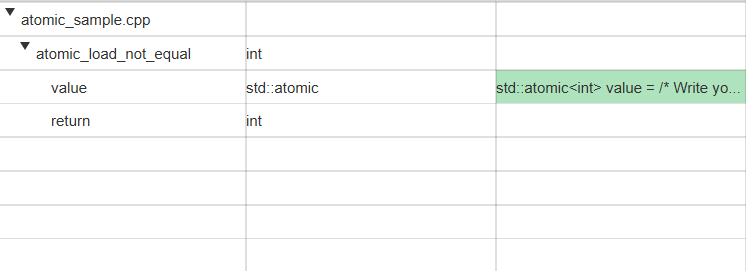
\includegraphics[width=0.9\textwidth]{images/atomic_begin.png}
    \caption{AKAUTAUTO chưa thể hiện được đúng trên Data Tree}
\end{figure}

Xuất phát từ thực trạng trên, báo cáo tập trung nghiên cứu và triển khai cơ chế hỗ trợ đối tượng \texttt{atomic} cho công cụ AKAUTAUTO. Các nội dung chính của đề tài bao gồm:

\begin{itemize}[leftmargin=*, itemsep=0.3em]
\item \textbf{Mở rộng mô hình dữ liệu:} Bổ sung cơ chế nhận diện và biểu diễn các đối tượng \texttt{atomic} trong quá trình phân tích cây cú pháp trừu tượng (AST).

\item \textbf{Hỗ trợ thực thi và đánh giá kiểm thử:} Cho phép người dùng khai báo giá trị kiểm thử cho các đối tượng \texttt{atomic}, thực thi chương trình và theo dõi kết quả độ phủ mã nguồn đối với các nhánh liên quan đến biến nguyên tử.

\end{itemize}

Kết quả đạt được góp phần mở rộng khả năng hỗ trợ của AKAUTAUTO đối với các chương trình sử dụng đối tượng \texttt{atomic}, tạo nền tảng cho việc nghiên cứu và phát triển các kỹ thuật sinh dữ liệu kiểm thử tự động cho môi trường đồng thời trong tương lai.



% =====================================================================
%  Chương 1: Kiến thức nền tảng
%  Nội dung: content/2.related_works.tex
% =====================================================================
\chapter{Kiến thức nền tảng}\label{Background}

% chktex-file 8
% chktex-file 24
% chktex-file 36
\section{Đối tượng \texttt{std::atomic} trong C++}

Thư viện chuẩn C++ cung cấp lớp mẫu \texttt{std::atomic} nhằm hỗ trợ các thao tác truy cập dữ liệu nguyên tử trong môi trường đa luồng~\cite{cppreference_atomic, williams2019cppconcurrency}. Một thao tác nguyên tử là thao tác được thực hiện như một đơn vị không thể bị chia cắt, bảo đảm rằng các luồng khác không thể quan sát trạng thái trung gian của dữ liệu trong quá trình thực thi. Nhờ đó, \texttt{std::atomic} được sử dụng rộng rãi để xây dựng các cơ chế đồng bộ hóa không khóa (lock-free synchronization), giúp giảm chi phí đồng bộ hóa và cải thiện hiệu năng của chương trình.

Đối tượng \texttt{std::atomic} được khai báo dưới dạng lớp mẫu với kiểu dữ liệu cơ sở là một kiểu nguyên thủy hoặc kiểu có thể sao chép đơn giản. Ví dụ, đoạn mã trong Liệt kê~\ref{lst:atomic_declare} minh họa cách khai báo một biến nguyên tử kiểu số nguyên.

\begin{lstlisting}[language=C++,caption={Khai báo đối tượng atomic},label={lst:atomic_declare}]
#include <atomic>

std::atomic<int> counter(0);
\end{lstlisting}

Khác với các biến thông thường, việc truy cập dữ liệu của đối tượng \texttt{atomic} thường được thực hiện thông qua các hàm thành viên chuyên biệt. Một số thao tác phổ biến bao gồm~\cite{cppreference_atomic}:

\begin{itemize}
\item \textbf{\texttt{load()}:} Đọc giá trị hiện tại của đối tượng nguyên tử.

\item \textbf{\texttt{store()}:} Ghi một giá trị mới vào đối tượng nguyên tử.

\item \textbf{\texttt{exchange()}:} Thay thế giá trị hiện tại bằng giá trị mới và trả về giá trị trước khi thay thế.

\item \textbf{Các thao tác \texttt{compare\_exchange}:} So sánh giá trị hiện tại với giá trị kỳ vọng. Hai biến thể phổ biến là \nolinkurl{compare_exchange_weak()} và \nolinkurl{compare_exchange_strong()}; nếu hai giá trị bằng nhau thì cập nhật giá trị mới, ngược lại trả về giá trị hiện tại.
\end{itemize}

Ví dụ trong Liệt kê~\ref{lst:atomic_ops} minh họa việc sử dụng một số thao tác nguyên tử cơ bản.

\begin{lstlisting}[language=C++,caption={Các thao tác nguyên tử phổ biến},label={lst:atomic_ops}]
std::atomic<int> value(10);

int current = value.load();

value.store(20);

int old_value = value.exchange(30);

int expected = 30;
bool result = value.compare_exchange_strong(expected, 40);
\end{lstlisting}

Trong các chương trình thực tế, kết quả của các thao tác nguyên tử thường được sử dụng trực tiếp trong các biểu thức điều kiện để điều khiển luồng thực thi. Do đó, việc hỗ trợ nhận diện và xử lý các đối tượng \texttt{atomic} có vai trò quan trọng đối với các công cụ kiểm thử tự động. Nếu không mô hình hóa chính xác các thao tác như \texttt{load()}, \texttt{store()} hoặc \texttt{compare\_exchange()}, công cụ sẽ gặp khó khăn trong việc xây dựng dữ liệu kiểm thử và đánh giá độ phủ đối với các nhánh mã phụ thuộc vào trạng thái của biến nguyên tử.

\section{Kiểm thử đơn vị}

Kiểm thử đơn vị (Unit Testing) là quá trình kiểm tra tính đúng đắn của các đơn vị chức năng nhỏ nhất trong chương trình, chẳng hạn như hàm hoặc phương thức~\cite{phamngochung2014testing}. Mỗi lần kiểm thử được thực hiện thông qua một hoặc nhiều ca kiểm thử (Test Case), bao gồm dữ liệu đầu vào, điều kiện thực hiện và kết quả mong đợi. Mục tiêu của kiểm thử đơn vị là phát hiện sớm các lỗi logic trong quá trình phát triển, từ đó nâng cao chất lượng và độ tin cậy của phần mềm. Để đánh giá hiệu quả của bộ kiểm thử, người ta thường sử dụng các chỉ số độ phủ mã nguồn (Code Coverage), phản ánh mức độ mà mã nguồn đã được thực thi bởi các ca kiểm thử. Ba tiêu chí phổ biến là độ phủ câu lệnh (Statement Coverage), đo tỷ lệ số câu lệnh đã được thực thi ít nhất một lần, và độ phủ nhánh (Branch Coverage) và MC/DC (Modified condition/decision coverage), đo tỷ lệ các nhánh điều kiện đã được kiểm thử. Trong phạm vi đề tài này, độ phủ câu lệnh, độ phủ nhánh và MC/DC được sử dụng để đánh giá hiệu quả hỗ trợ kiểm thử đối với các chương trình sử dụng đối tượng \texttt{std::atomic}.


\section{Tổng quan dự án AKAUTAUTO}

AKAUTAUTO là công cụ hỗ trợ kiểm thử đơn vị tự động cho các chương trình C/C++, được phát triển bởi Phòng thí nghiệm Đảm bảo chất lượng phần mềm, Trường Đại học Công nghệ - Đại học Quốc gia Hà Nội, phối hợp cùng đơn vị FPT Global Automotive \& Manufacturing (FPT-GAM). Mục tiêu của dự án là hỗ trợ người kiểm thử xây dựng và thực thi các ca kiểm thử một cách hiệu quả, từ đó nâng cao chất lượng phần mềm và giảm chi phí kiểm thử thủ công.

Hệ thống được xây dựng dựa trên kỹ thuật thực thi tượng trưng động, kết hợp giữa thực thi cụ thể và phân tích tượng trưng để khám phá các đường thực thi trong chương trình~\cite{nguyenducanh2015,sen2005cute}. Thông qua việc phân tích mã nguồn C/C++, công cụ có khả năng xây dựng mô hình chương trình, thu thập các điều kiện rẽ nhánh, tạo dữ liệu kiểm thử và đánh giá độ phủ mã nguồn của các ca kiểm thử đã thực hiện.

Kiến trúc của AKAUTAUTO bao gồm nhiều thành phần chức năng liên kết với nhau. Đầu tiên, mã nguồn được phân tích bằng bộ phân tích cú pháp để xây dựng Cây cú pháp trừu tượng (Abstract Syntax Tree - AST) và các cấu trúc biểu diễn chương trình liên quan. Từ AST, hệ thống trích xuất thông tin về hàm cần kiểm thử, tham số đầu vào, kiểu dữ liệu và các điều kiện điều khiển luồng thực thi. Tiếp theo, công cụ xây dựng cây dữ liệu kiểm thử (Data Tree) nhằm biểu diễn các biến đầu vào dưới dạng cấu trúc có thể cấu hình và quản lý. Dựa trên thông tin thu thập được, hệ thống sinh mã kiểm thử (test driver), biên dịch chương trình và thực thi các ca kiểm thử tương ứng.

Ngoài khả năng hỗ trợ sinh dữ liệu kiểm thử, AKAUTAUTO còn cung cấp các chức năng đánh giá kết quả thực thi và hiển thị trực quan các vùng mã nguồn đã hoặc chưa được kiểm thử. Những thông tin này giúp người phát triển xác định các khu vực cần bổ sung dữ liệu kiểm thử để nâng cao chất lượng kiểm thử tổng thể.

Qua nhiều giai đoạn phát triển, AKAUTAUTO đã hỗ trợ nhiều kiểu dữ liệu và cơ chế kiểm thử khác nhau trong ngôn ngữ C/C++. Tuy nhiên, một số kiểu dữ liệu đặc biệt của thư viện chuẩn C++, chẳng hạn như \texttt{std::atomic}, vẫn chưa được hỗ trợ đầy đủ trong mô hình dữ liệu và quy trình kiểm thử của hệ thống. Đây cũng chính là động lực cho nghiên cứu mở rộng được trình bày trong báo cáo này.


\section{Mô hình node dữ liệu cho các cấu trúc dữ liệu chuẩn \texttt{STL} trong AKAUTAUTO}

Trong AKAUTAUTO, dữ liệu kiểm thử được biểu diễn dưới dạng cây dữ liệu, trong đó mỗi nút mô tả một biến, một trường dữ liệu hoặc một thành phần con của đối tượng cần kiểm thử. Đối với các kiểu dữ liệu cơ bản như \texttt{int}, \texttt{float}, \texttt{char} hoặc \texttt{bool}, hệ thống có thể biểu diễn trực tiếp thông qua các nút dữ liệu giá trị. Tuy nhiên, với các kiểu dữ liệu phức tạp hơn, đặc biệt là các kiểu thuộc thư viện chuẩn C++ như \texttt{std::vector}, \texttt{std::string} hoặc \texttt{std::map}, việc biểu diễn trực tiếp dưới dạng một giá trị đơn lẻ là không phù hợp. Do đó, AKAUTAUTO sử dụng mô hình \texttt{STLDataNode} để mô tả các đối tượng thuộc Standard Template Library (STL).

\texttt{STLDataNode} đóng vai trò là lớp biểu diễn trung gian cho các kiểu dữ liệu STL trong cây dữ liệu kiểm thử. Thay vì coi một đối tượng STL là một biến nguyên thủy, hệ thống phân rã đối tượng đó thành các thành phần có thể quản lý được, chẳng hạn như kích thước container, kiểu phần tử và danh sách các phần tử con. Cách biểu diễn này giúp người dùng có thể quan sát, cấu hình và nhập dữ liệu kiểm thử cho các đối tượng STL thông qua giao diện cây dữ liệu.

Ví dụ, với một biến kiểu \texttt{std::vector<int>}, hệ thống không chỉ lưu thông tin rằng biến có kiểu \texttt{std::vector<int>}, mà còn cần xác định số lượng phần tử và tạo ra các nút con tương ứng với từng phần tử trong vector. Mỗi phần tử con sau đó có thể được biểu diễn bằng một nút dữ liệu giá trị kiểu \texttt{int}. Nhờ đó, quá trình sinh test driver có thể khởi tạo lại đối tượng \texttt{std::vector<int>} bằng các giá trị mà người dùng đã cung cấp.

\begin{lstlisting}[language=C++,caption={Ví dụ khai báo đối tượng STL},label={lst:stl_vector_example}]
#include <vector>

void foo(std::vector<int> values) {
    if (values.size() > 0 && values[0] > 10) {
        // ...
    }
}
\end{lstlisting}

Với đoạn mã trên, cây dữ liệu kiểm thử có thể biểu diễn biến \texttt{values} như một nút \texttt{STLDataNode}. Nút này chứa thông tin về kiểu container là \texttt{std::vector}, kiểu phần tử là \texttt{int}, đồng thời quản lý các nút con tương ứng với từng phần tử của vector. Khi người dùng thiết lập kích thước và giá trị cho các phần tử, hệ thống có thể sinh mã khởi tạo tương ứng trong test driver.

\begin{lstlisting}[language=C++,caption={Ví dụ mã khởi tạo dữ liệu kiểm thử cho vector},label={lst:stl_vector_init}]
std::vector<int> values;
values.push_back(15);
\end{lstlisting}

Mô hình \texttt{STLDataNode} cho thấy cách AKAUTAUTO xử lý các kiểu dữ liệu không nguyên thủy bằng cách xây dựng một lớp biểu diễn riêng trong cây dữ liệu. Đây là cơ sở quan trọng để mở rộng hệ thống sang các kiểu dữ liệu đặc biệt khác. Trong phạm vi đề tài này, ý tưởng tương tự được áp dụng để xây dựng cơ chế hỗ trợ đối tượng \texttt{std::atomic}. Tuy nhiên, khác với các container STL, đối tượng \texttt{atomic} không biểu diễn một tập hợp phần tử mà bao bọc một giá trị cơ sở và cung cấp các thao tác truy cập nguyên tử như \texttt{load()}, \texttt{store()}, \texttt{exchange()} và \texttt{compare\_exchange()}. Vì vậy, việc hỗ trợ \texttt{atomic} cần một mô hình dữ liệu riêng, vừa kế thừa cách tổ chức của cây dữ liệu trong AKAUTAUTO, vừa bổ sung khả năng nhận diện kiểu dữ liệu cơ sở và sinh mã khởi tạo phù hợp cho đối tượng nguyên tử.

\section{Cây cú pháp trừu tượng trong phân tích mã nguồn C/C++}

Cây cú pháp trừu tượng (Abstract Syntax Tree - AST) là cấu trúc dạng cây biểu diễn thành phần cú pháp của chương trình sau quá trình phân tích mã nguồn~\cite{phamngochung2014ut}. Trong AST, mỗi nút tương ứng với một thành phần của chương trình, chẳng hạn như khai báo biến, lời gọi hàm, biểu thức điều kiện, câu lệnh gán hoặc định nghĩa hàm. So với mã nguồn dạng văn bản, AST giúp công cụ phân tích chương trình dễ dàng truy xuất thông tin về kiểu dữ liệu, tên biến, danh sách tham số và cấu trúc điều khiển.

Trong AKAUTAUTO, AST được sử dụng ở giai đoạn đầu của quy trình kiểm thử nhằm trích xuất thông tin cần thiết từ mã nguồn C/C++. Từ AST, hệ thống có thể xác định hàm cần kiểm thử, các tham số đầu vào, kiểu dữ liệu của từng biến và các biểu thức điều kiện xuất hiện trong thân hàm. Những thông tin này là cơ sở để xây dựng cây dữ liệu kiểm thử, sinh test driver và đánh giá độ phủ mã nguồn.

Đối với đề tài này, AST đóng vai trò quan trọng trong việc nhận diện các biến có kiểu \texttt{std::atomic}. Thay vì chỉ xử lý các kiểu dữ liệu cơ bản như \texttt{int}, \texttt{float} hoặc \texttt{bool}, hệ thống cần phân tích kiểu dữ liệu dạng mẫu như \texttt{std::atomic<T>} để xác định kiểu dữ liệu cơ sở \texttt{T}. Việc nhận diện chính xác kiểu \texttt{atomic} trong AST là bước đầu tiên để ánh xạ biến nguyên tử sang mô hình \texttt{AtomicDataNode} trong cây dữ liệu kiểm thử.

\section{Test driver và stub trong AKAUTAUTO}

Trong kiểm thử đơn vị, test driver là đoạn mã được sinh ra để khởi tạo dữ liệu đầu vào, gọi hàm cần kiểm thử và thu thập kết quả thực thi~\cite{nguyenducanh2015}. Đối với AKAUTAUTO, test driver được tạo tự động dựa trên cây dữ liệu kiểm thử do người dùng hoặc hệ thống thiết lập. Mỗi biến đầu vào trong Data Tree sẽ được chuyển thành các câu lệnh khai báo và khởi tạo tương ứng trong mã kiểm thử.

Bên cạnh test driver, stub được sử dụng để thay thế hoặc mô phỏng hành vi của các hàm phụ thuộc trong quá trình kiểm thử~\cite{trannguyenhuong2022stub}. Khi hàm cần kiểm thử gọi đến một hàm khác chưa được kiểm thử trực tiếp, hệ thống có thể sinh stub nhằm kiểm soát giá trị trả về hoặc trạng thái dữ liệu liên quan. Cơ chế này giúp cô lập đơn vị cần kiểm thử và giảm sự phụ thuộc vào các thành phần bên ngoài.

Trong ngữ cảnh hỗ trợ \texttt{std::atomic}, cả test driver và stub đều cần được điều chỉnh để sinh mã phù hợp với ngữ nghĩa của đối tượng nguyên tử. Khác với các biến thông thường, \texttt{std::atomic} không nên được xử lý bằng phép gán trực tiếp trong một số ngữ cảnh sinh mã. Thay vào đó, hệ thống cần sử dụng \texttt{store()} để ghi giá trị và \texttt{load()} để đọc giá trị hiện tại. Đây là cơ sở cho việc mở rộng cơ chế sinh mã kiểm thử và khắc phục lỗi biên dịch khi xử lý các tham số hoặc biến có kiểu \texttt{std::atomic}.

\section{Tổng quan về công cụ VectorCAST}

VectorCAST là một công cụ kiểm thử đơn vị thương mại dành cho các ngôn ngữ C và C++, được phát triển bởi Vector Software~\cite{vectorcast2025}. Công cụ hỗ trợ tự động xây dựng môi trường kiểm thử, sinh test driver, quản lý dữ liệu kiểm thử, thực thi test case và thu thập các chỉ số độ bao phủ mã nguồn như Statement Coverage, Branch Coverage, MC/DC và Function Coverage. Nhờ khả năng tích hợp với nhiều trình biên dịch và môi trường phát triển khác nhau, VectorCAST được sử dụng rộng rãi trong các lĩnh vực yêu cầu độ tin cậy cao như ô tô, hàng không và hệ thống nhúng.

Quy trình kiểm thử trong VectorCAST bắt đầu bằng việc lựa chọn đơn vị kiểm thử (Unit Under Test - UUT), sau đó công cụ phân tích mã nguồn để xây dựng mô hình dữ liệu của các tham số đầu vào, biến toàn cục và giá trị trả về. Dựa trên mô hình này, người dùng có thể tạo và quản lý các bộ dữ liệu kiểm thử thông qua giao diện đồ họa mà không cần viết mã kiểm thử thủ công.

Tuy nhiên, kết quả thực nghiệm cho thấy việc hỗ trợ các kiểu dữ liệu hiện đại của C++ vẫn còn một số hạn chế. Đối với kiểu dữ liệu \texttt{std::atomic<T>}, VectorCAST không tự động nhận diện và sinh dữ liệu kiểm thử tương ứng như đối với các kiểu nguyên thủy hoặc cấu trúc dữ liệu thông thường. Thay vào đó, tham số kiểu \texttt{std::atomic<T>} được hiển thị dưới dạng \textit{user-defined parameter} và yêu cầu người dùng tự cung cấp mã khởi tạo thông qua cơ chế \textit{User Code}. Điều này cho thấy công cụ chưa xây dựng được mô hình dữ liệu nội bộ cho đối tượng atomic và chưa hỗ trợ tự động sinh dữ liệu kiểm thử cho kiểu dữ liệu này.

Hình~\ref{fig:VectorCAST} minh họa trường hợp VectorCAST không thể tự động gán giá trị cho tham số kiểu \texttt{std::atomic<int>} và yêu cầu người dùng nhập mã khởi tạo thủ công.

\begin{figure}[H]
\centering
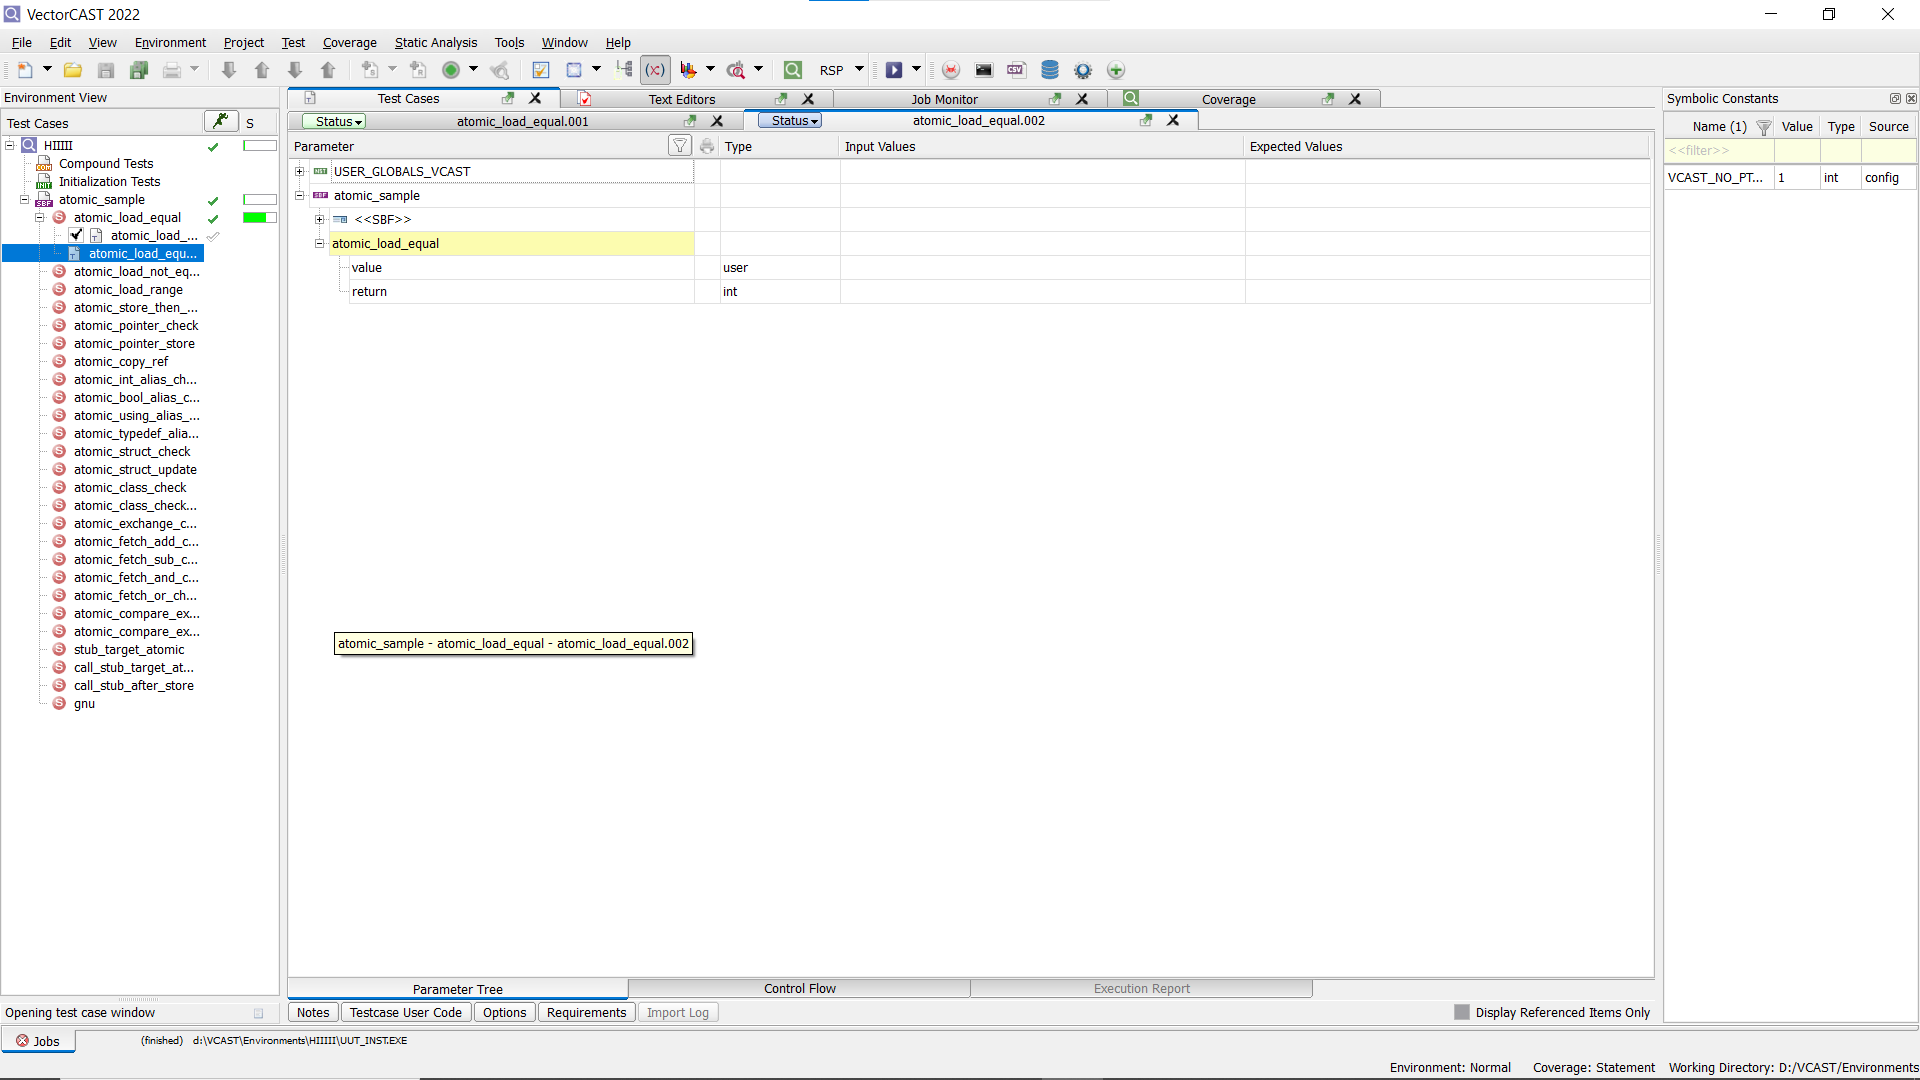
\includegraphics[width=0.9\linewidth]{images/VectorCAST.png}
\caption[VectorCAST yêu cầu nhập mã khởi tạo thủ công]{VectorCAST yêu cầu nhập mã khởi tạo thủ công cho tham số \texttt{std::atomic}}
\label{fig:VectorCAST}
\end{figure}


% =====================================================================
%  Chương 2: Phương pháp đề xuất
%  Nội dung: content/3.methodology.tex
% =====================================================================
\chapter{Phương pháp đề xuất}\label{Method}

% chktex-file 13
Để hỗ trợ kiểm thử các chương trình sử dụng đối tượng \texttt{std::atomic}, nghiên cứu đề xuất mở rộng cơ chế biểu diễn dữ liệu và sinh mã kiểm thử trong công cụ AKAUTAUTO. Trong phiên bản hiện tại, hệ thống đã hỗ trợ nhiều kiểu dữ liệu cơ bản và một số cấu trúc dữ liệu thuộc thư viện STL. Tuy nhiên, các đối tượng \texttt{std::atomic} chưa được nhận diện và xử lý đầy đủ trong quá trình xây dựng cây dữ liệu kiểm thử cũng như sinh test driver. Điều này khiến công cụ gặp khó khăn khi làm việc với các hàm có tham số hoặc biến sử dụng kiểu dữ liệu nguyên tử.

% chktex-file 1
% chktex-file 24
% chktex-file 36
Giải pháp đề xuất gồm ba nội dung chính:

\begin{enumerate}
    \item Nhận diện kiểu dữ liệu \texttt{std::atomic} trong quá trình phân tích mã nguồn.

    \item Xây dựng lớp \texttt{AtomicDataNode} để biểu diễn đối tượng nguyên tử trong cây dữ liệu kiểm thử.

    \item Mở rộng cơ chế sinh test driver nhằm hỗ trợ khởi tạo và xử lý các đối tượng \texttt{atomic}.
\end{enumerate}


\section{Nhận diện kiểu dữ liệu \texttt{atomic}}

Trong phiên bản gốc, AKAUTAUTO hỗ trợ một số kiểu dữ liệu thuộc thư viện STL như \texttt{vector}, \texttt{set}, \texttt{map}, \texttt{queue} và các smart pointer. Khi phân tích mã nguồn, hệ thống dựa trên thông tin kiểu dữ liệu thu được từ AST để xác định lớp DataNode tương ứng.

Để hỗ trợ \texttt{std::atomic}, hệ thống được mở rộng bằng cách bổ sung kiểu \texttt{atomic} vào danh sách các kiểu STL được nhận diện. Khi gặp một biến kiểu \texttt{std::atomic} với tham số mẫu \texttt{T}, hệ thống xác định \texttt{T} là kiểu dữ liệu cơ sở và chuyển sang cơ chế xử lý riêng thay vì coi đây là một biến thông thường.

Việc nhận diện chính xác kiểu \texttt{atomic} là điều kiện tiên quyết để xây dựng mô hình dữ liệu phù hợp cũng như sinh mã kiểm thử chính xác cho các đối tượng nguyên tử.

\section{Thiết kế lớp \texttt{AtomicDataNode}}

Sau khi nhận diện được kiểu dữ liệu \texttt{std::atomic}, nghiên cứu xây dựng lớp \texttt{AtomicDataNode} kế thừa từ \texttt{STLDataNode} để biểu diễn đối tượng nguyên tử trong Data Tree.

Việc kế thừa từ \texttt{STLDataNode} cho phép tái sử dụng cơ chế quản lý dữ liệu và tổ chức cây dữ liệu đã được triển khai trong \textit{AKAUTAUTO}, đồng thời hạn chế tối đa các thay đổi đối với kiến trúc hiện có của hệ thống.

Khác với các container STL như \texttt{vector}, \texttt{list} hay \texttt{map}, \texttt{std::atomic} chỉ bao bọc một giá trị cơ sở duy nhất. Do đó, mỗi đối tượng \texttt{atomic} được biểu diễn bởi một nút \texttt{AtomicDataNode} chứa một nút con lưu trữ giá trị thực của kiểu dữ liệu cơ sở.

\begin{figure}[H]
\centering
\begin{forest}
for tree={
draw,
rounded corners,
align=center,
parent anchor=south,
child anchor=north
}
[{AtomicDataNode\\\texttt{atomic<int>}}
  [{ValueDataNode\\\texttt{10}}]
]
\end{forest}
\caption{Mô hình biểu diễn đối tượng atomic trong Data Tree}
\label{fig:atomic_data_tree}
\end{figure}

Hình~\ref{fig:atomic_data_tree} minh họa cách biểu diễn đối tượng \texttt{std::atomic<int>} trong cây dữ liệu kiểm thử. Nút \texttt{AtomicDataNode} đóng vai trò là lớp bao ngoài của đối tượng nguyên tử, trong khi nút con \texttt{ValueDataNode} lưu trữ giá trị thực của kiểu dữ liệu cơ sở. Cách biểu diễn này cho phép người dùng cấu hình dữ liệu kiểm thử cho đối tượng \texttt{atomic} tương tự như các kiểu dữ liệu đã được hỗ trợ trước đó.

\section{Sinh test driver cho đối tượng \texttt{atomic}}

Sau khi xây dựng được mô hình \texttt{AtomicDataNode}, hệ thống cần sinh mã khởi tạo tương ứng trong test driver. Quá trình này được thực hiện dựa trên thông tin lưu trữ trong Data Tree, bao gồm kiểu dữ liệu cơ sở và giá trị do người dùng cung cấp.

Thuật toán sinh mã được thực hiện theo các bước sau:

\begin{algorithm}[H]
\caption{Sinh mã kiểm thử cho đối tượng \texttt{std::atomic}}
\label{alg:atomic-driver-generation}
\begin{algorithmic}[1]
\Require Nút dữ liệu \texttt{AtomicDataNode} biểu diễn đối tượng \texttt{std::atomic<T>}
\Ensure Đoạn mã khởi tạo đối tượng \texttt{atomic} trong test driver

\State Trích xuất kiểu dữ liệu cơ sở \texttt{T} từ kiểu \texttt{std::atomic<T>}
\State Lấy tên biến kiểm thử từ \texttt{AtomicDataNode}
\State Lấy nút con biểu diễn giá trị thực của kiểu \texttt{T}
\State Sinh mã khai báo biến \texttt{std::atomic<T>}
\If{nút con có giá trị kiểm thử}
    \State Sinh biến tạm lưu giá trị kiểu \texttt{T}
    \State Sinh câu lệnh \texttt{atomicVar.store(value)}
\Else
    \State Bỏ qua bước khởi tạo giá trị cho đối tượng \texttt{atomic}
\EndIf
\State Trả về đoạn mã kiểm thử đã sinh
\end{algorithmic}
\end{algorithm}

Ví dụ, đối với cấu trúc dữ liệu trong Hình~\ref{fig:atomic_data_tree}, hệ thống sẽ sinh đoạn mã kiểm thử:

\begin{lstlisting}[language=C++,caption={Ví dụ khai báo đối tượng std::atomic trong test driver},label={lst:std_atomic_example}]
std::atomic<int> value;
int value_AtomicValue = 10;
value.store(value_AtomicValue);
\end{lstlisting}

Việc sử dụng phương thức \texttt{store()} thay cho phép gán trực tiếp giúp mã kiểm thử tuân thủ ngữ nghĩa của thư viện \texttt{std::atomic} và bảo đảm khả năng biên dịch trong môi trường C++.

\section{Điều chỉnh cơ chế xử lý stub đối với \texttt{atomic}}

Trong AKAUTAUTO, quá trình sinh test driver và stub thường yêu cầu sao chép dữ liệu giữa các biến~\cite{trannguyenhuong2022stub}. Đối với các kiểu dữ liệu thông thường, việc sao chép được thực hiện thông qua phép gán trực tiếp:

\begin{lstlisting}[language=C++,caption={Ví dụ khai báo đối tượng stub},label={lst:stub_example}]
int dest;
int AKA_stub_1 = 3;

dest = AKA_stub_1;
\end{lstlisting}

Tuy nhiên, cách tiếp cận này không phù hợp đối với các đối tượng \texttt{std::atomic}. Việc sử dụng phép gán trực tiếp trong một số ngữ cảnh sinh mã có thể dẫn đến lỗi biên dịch hoặc không phản ánh đúng cơ chế truy cập dữ liệu nguyên tử của thư viện chuẩn C++.

Để khắc phục hạn chế này, hệ thống được điều chỉnh để sử dụng cặp thao tác \texttt{load()} và \texttt{store()} khi xử lý các đối tượng nguyên tử. Cụ thể, giá trị hiện tại của đối tượng nguồn được lấy thông qua \texttt{load()} và sau đó được ghi vào đối tượng đích bằng \texttt{store()}:

\begin{lstlisting}[language=C++,caption={Ví dụ sử dụng stub với đối tượng std::atomic},label={lst:std_atomic_stub_example}]
std::atomic<int> AKA_STUB_value;
std::atomic<int> dest;
int AKA_STUB_value_AtomicValue = 5;
AKA_STUB_value.store(AKA_STUB_value_AtomicValue);
dest.store(AKA_STUB_value.load());
\end{lstlisting}

Cách tiếp cận này bảo đảm việc sao chép dữ liệu giữa các đối tượng \texttt{atomic} tuân thủ đúng ngữ nghĩa của thư viện chuẩn, đồng thời giúp các đoạn mã được sinh ra có thể biên dịch và thực thi thành công. Đây cũng là bước cần thiết để hỗ trợ đầy đủ các tham số và biến có kiểu \texttt{std::atomic} trong quá trình kiểm thử.

\section{Quy trình kiểm thử hỗ trợ \texttt{atomic}}

Sau khi bổ sung cơ chế hỗ trợ \texttt{atomic}, quy trình kiểm thử của hệ thống bao gồm các bước:

\begin{enumerate}
\item Phân tích AST và nhận diện đối tượng \texttt{std::atomic}.
\item Xây dựng Data Tree chứa nút \texttt{AtomicDataNode}.
\item Cho phép người dùng nhập giá trị kiểm thử cho đối tượng nguyên tử.
\item Sinh test driver tương ứng.
\item Biên dịch và thực thi chương trình kiểm thử.
\item Thu thập và hiển thị kết quả độ phủ mã nguồn.
\end{enumerate}

\begin{figure}[H]
\centering

\begin{forest}
for tree={
draw,
rounded corners,
align=center,
minimum width=4cm
}
[C/C++ Source Code
    [AST Analysis\\Detect \texttt{std::atomic<T>}
        [Data Tree Construction\\\texttt{AtomicDataNode}
            [User Input Test Data
                [{Test Driver Generation\\\texttt{store()}, \texttt{load()}}
                    [Compile \& Execute
                        [Coverage Collection
                            [Coverage Report]
                        ]
                    ]
                ]
            ]
        ]
    ]
]
\end{forest}

\caption{Quy trình hỗ trợ đối tượng \texttt{std::atomic} trong AKAUTAUTO}
\label{fig:atomic_workflow}

\end{figure}

Giải pháp đề xuất giúp AKAUTAUTO hỗ trợ các đối tượng \texttt{std::atomic} trong toàn bộ quy trình kiểm thử hiện tại, từ giai đoạn phân tích mã nguồn, xây dựng cây dữ liệu, sinh test driver đến thực thi chương trình kiểm thử và thu thập độ phủ mã nguồn. Qua đó, phạm vi hỗ trợ của công cụ được mở rộng đối với các chương trình C/C++ sử dụng kiểu dữ liệu nguyên tử.



% =====================================================================
%  Chương 3: Thực nghiệm
%  Nội dung: content/4.experimental_result.tex
% =====================================================================
\chapter{Thực nghiệm}\label{Experiments}

% chktex-file 1
% chktex-file 13
% chktex-file 24
% chktex-file 36
\section{Mục tiêu thực nghiệm}

Mục tiêu của quá trình thực nghiệm là đánh giá tính đúng đắn và hiệu quả của cơ chế hỗ trợ đối tượng \texttt{std::atomic} được bổ sung vào công cụ AKAUTAUTO. Thực nghiệm tập trung kiểm chứng khả năng của hệ thống trong việc nhận diện chính xác các biến có kiểu \texttt{std::atomic}, xây dựng cây dữ liệu kiểm thử tương ứng và sinh mã kiểm thử có thể biên dịch, thực thi thành công.

Bên cạnh đó, thực nghiệm đánh giá tính chính xác của lớp \texttt{AtomicDataNode} trong việc biểu diễn dữ liệu nguyên tử, cho phép người dùng cấu hình giá trị kiểm thử và sinh mã khởi tạo phù hợp trong test driver. Một mục tiêu quan trọng khác là kiểm chứng cơ chế xử lý các thao tác \texttt{load()} và \texttt{store()} trong quá trình sinh mã kiểm thử, bảo đảm các đoạn mã được sinh ra tuân thủ ngữ nghĩa của \texttt{std::atomic}.

Cuối cùng, thực nghiệm đánh giá mức độ cải thiện về khả năng kiểm thử thông qua các chỉ số độ phủ mã nguồn. Kết quả thu được được sử dụng để xác nhận rằng giải pháp đề xuất giúp mở rộng phạm vi hỗ trợ của AKAUTAUTO đối với các chương trình C/C++ sử dụng đối tượng nguyên tử.

\section{Cài đặt công cụ}

Công cụ được cài đặt và tích hợp dựa trên kiến trúc hiện có của AKAUTAUTO. Kiến trúc tổng quan của hệ thống bao gồm năm mô-đun chính: mô-đun xây dựng môi trường kiểm thử, mô-đun phân tích mã nguồn, mô-đun sinh dữ liệu kiểm thử, mô-đun thực thi và phân tích ca kiểm thử, và mô-đun sinh báo cáo kết quả. Trong phạm vi đề tài này, các cải tiến tập trung vào mô-đun phân tích mã nguồn, cây dữ liệu kiểm thử và cơ chế sinh test driver cho đối tượng \texttt{std::atomic}.

\begin{figure}[H]
    \centering
    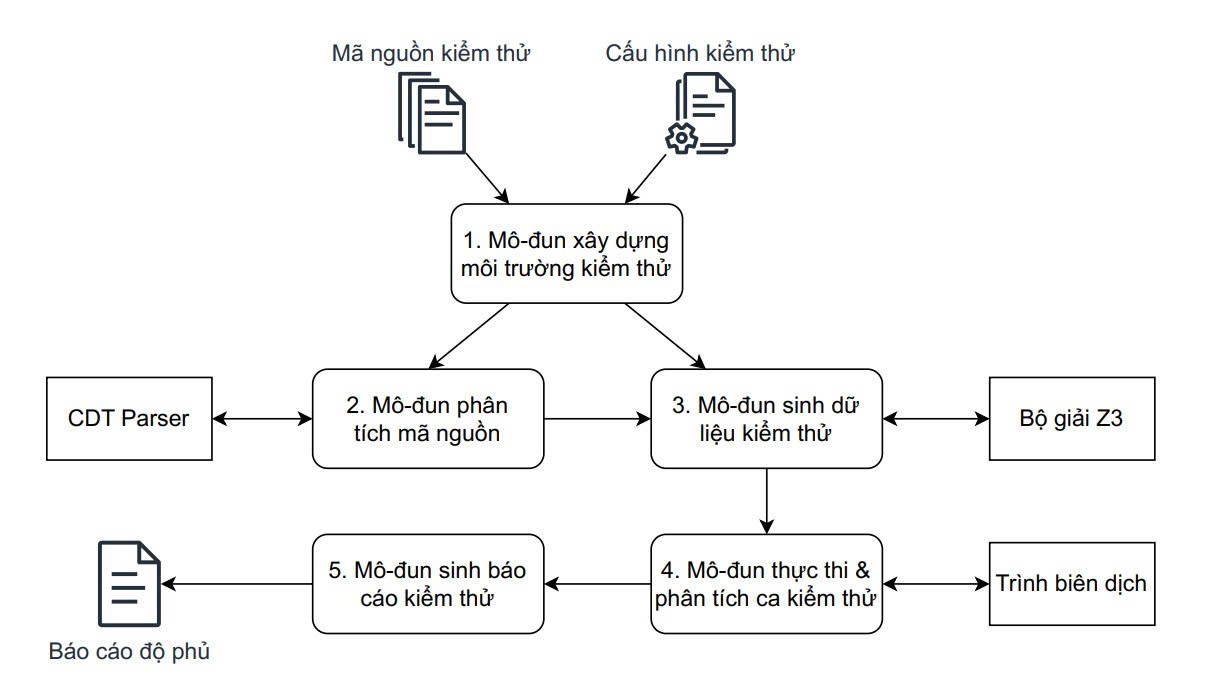
\includegraphics[width=0.95\linewidth]{images/image.png}
    \caption{Kiến trúc công cụ AKAUTAUTO}
    \label{fig:akautauto_architecture}
\end{figure}

\section[Công cụ AKAUTAUTO sau khi hỗ trợ \texttt{std::atomic}]{Công cụ AKAUTAUTO sau khi hỗ trợ\\\texttt{std::atomic}}

Sau khi bổ sung cơ chế hỗ trợ đối tượng \texttt{std::atomic}, kiến trúc tổng thể của công cụ AKAUTAUTO vẫn được giữ nguyên, tuy nhiên khả năng xử lý các chương trình C++ sử dụng kiểu dữ liệu nguyên tử đã được mở rộng. Các thành phần cốt lõi như bộ phân tích mã nguồn, cây dữ liệu kiểm thử (Data Tree), bộ sinh test driver và mô-đun đánh giá độ phủ vẫn được kế thừa từ phiên bản trước. Những thay đổi chủ yếu tập trung vào quá trình nhận diện kiểu dữ liệu và sinh mã kiểm thử cho các đối tượng \texttt{atomic}.

Cụ thể, mô-đun phân tích mã nguồn đã được mở rộng để nhận diện các biến có kiểu \texttt{std::atomic} với kiểu dữ liệu cơ sở tương ứng trong quá trình duyệt cây cú pháp trừu tượng (AST). Sau khi phát hiện kiểu dữ liệu nguyên tử, hệ thống tự động ánh xạ đối tượng sang lớp \texttt{AtomicDataNode} trong cây dữ liệu kiểm thử. Điều này cho phép các đối tượng \texttt{atomic} được quản lý và cấu hình dữ liệu đầu vào tương tự các kiểu dữ liệu đã được hỗ trợ trong hệ thống.

\begin{figure}[htbp]
    \centering
    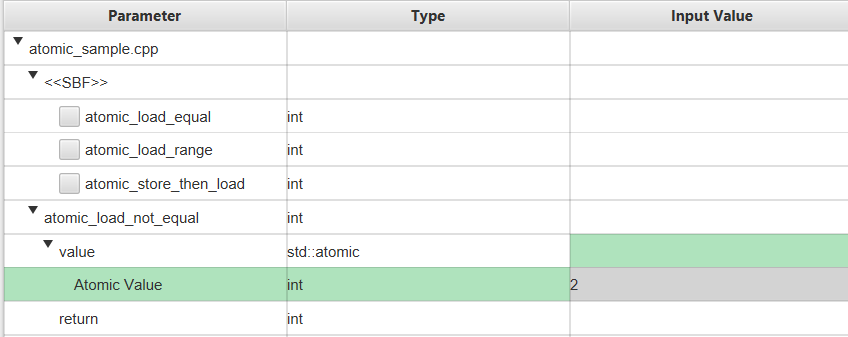
\includegraphics[width=0.9\textwidth]{images/atomic_after.png}
    \caption{AKAUTAUTO đã có thể nhận biết được trên Data Tree}
\end{figure}

Bên cạnh đó, cơ chế sinh test driver cũng được điều chỉnh nhằm xử lý đúng ngữ nghĩa của thư viện \texttt{std::atomic}. Thay vì sử dụng phép gán trực tiếp như đối với các kiểu dữ liệu thông thường, hệ thống sinh các câu lệnh \texttt{store()} để khởi tạo giá trị và sử dụng cặp thao tác \texttt{load()}--\texttt{store()} khi cần sao chép dữ liệu giữa các đối tượng nguyên tử. Nhờ đó, các đoạn mã kiểm thử được sinh ra có thể biên dịch và thực thi thành công đối với các hàm có tham số hoặc biến sử dụng \texttt{std::atomic}.

Kết quả thực nghiệm cho thấy phiên bản mở rộng của AKAUTAUTO có khả năng xử lý thành công các chương trình sử dụng \texttt{std::atomic}, bao gồm các trường hợp truyền tham chiếu, con trỏ, bí danh kiểu dữ liệu và các thao tác nguyên tử phổ biến như \texttt{load()}, \texttt{store()}, \texttt{exchange()} và \texttt{compare\_exchange()}.

\section{Dữ liệu và quy trình thực nghiệm}

\subsection{Dữ liệu thực nghiệm}

Để đánh giá tính đúng đắn của cơ chế hỗ trợ \texttt{std::atomic}, nghiên cứu xây dựng một bộ chương trình C++ thực nghiệm gồm 25 hàm sử dụng đối tượng nguyên tử dưới nhiều hình thức khác nhau. Các hàm được thiết kế nhằm kiểm tra khả năng nhận diện kiểu dữ liệu, xây dựng cây dữ liệu kiểm thử, sinh test driver và thực thi kiểm thử của hệ thống.

Bộ thực nghiệm được chia thành các nhóm chính bao gồm:

\begin{itemize}
\item Nhóm sử dụng các thao tác cơ bản \texttt{load()} và \texttt{store()}.
\item Nhóm sử dụng tham chiếu và con trỏ tới đối tượng \texttt{std::atomic}.
\item Nhóm sử dụng các bí danh kiểu dữ liệu như \texttt{std::atomic\_int}, \texttt{typedef} và \texttt{using}.
\item Nhóm sử dụng \texttt{std::atomic} làm thành viên của \texttt{struct} hoặc \texttt{class}.
\item Nhóm sử dụng các thao tác nguyên tử mở rộng như \texttt{exchange()}, nhóm \nolinkurl{fetch_*} và \nolinkurl{compare_exchange()}.
\item Nhóm kiểm thử cơ chế sinh stub và xử lý tham số kiểu \texttt{std::atomic}.
\end{itemize}

Các chương trình thực nghiệm được sử dụng để kiểm tra khả năng nhận diện đối tượng nguyên tử trong AST, xây dựng \texttt{AtomicDataNode}, sinh mã kiểm thử và thu thập kết quả độ phủ mã nguồn sau khi thực thi.


\subsection{Quy trình thực nghiệm}

\begin{table}[H]
\centering
\caption{Quy trình thực nghiệm nhận diện và biểu diễn \texttt{std::atomic}}
\label{tab:atomic-datanode-testing}
\renewcommand{\arraystretch}{1.3}
\begin{tabular}{@{}L{4cm}L{9cm}@{}}
\toprule
\multicolumn{2}{c}{\textbf{Testing Summary}} \\
\midrule
\textbf{Module} & Nhận diện \texttt{std::atomic} và xây dựng \texttt{AtomicDataNode} \\
\midrule
\textbf{Input} & Source code chứa biến hoặc tham số kiểu \texttt{std::atomic} \\
\midrule
\textbf{Expected output} &
\begin{minipage}[t]{\linewidth}
\raggedright
\vspace{-0.65\baselineskip}
\begin{itemize}
    \setlength{\itemsep}{2pt}
    \setlength{\parskip}{0pt}
    \setlength{\topsep}{0pt}
    \item Nhận diện đúng đối tượng \texttt{std::atomic}
    \item Tạo nút \texttt{AtomicDataNode} trong Data Tree
    \item Cho phép cấu hình giá trị kiểm thử cho kiểu dữ liệu cơ sở
\end{itemize}
\vspace{0.1\baselineskip}
\end{minipage} \\
\midrule
\textbf{Quy trình thực hiện} &
\begin{minipage}[t]{\linewidth}
\raggedright
\vspace{-0.65\baselineskip}
\begin{enumerate}
    \setlength{\itemsep}{2pt}
    \setlength{\parskip}{0pt}
    \setlength{\topsep}{0pt}
    \item Build môi trường kiểm thử
    \item Phân tích mã nguồn và xây dựng Data Tree
    \item Kiểm tra kiểu node được sinh ra cho đối tượng \texttt{atomic}
\end{enumerate}
\vspace{0.1\baselineskip}
\end{minipage} \\
\bottomrule
\end{tabular}
\end{table}

\textbf{Kịch bản 1: Nhận diện và biểu diễn đối tượng \texttt{std::atomic}.} Trong kịch bản này, dữ liệu đầu vào là các tệp mã nguồn có chứa biến hoặc tham số kiểu \texttt{std::atomic}. Hệ thống được kỳ vọng nhận diện đúng kiểu dữ liệu nguyên tử trong quá trình phân tích AST, xác định kiểu dữ liệu cơ sở và tạo nút \texttt{AtomicDataNode} tương ứng trong Data Tree. Người dùng sau đó có thể cấu hình giá trị kiểm thử cho đối tượng nguyên tử trên giao diện của công cụ.

\begin{table}[H]
\centering
\caption{Quy trình thực nghiệm sinh mã kiểm thử cho \texttt{std::atomic}}
\label{tab:atomic-driver-testing}
\renewcommand{\arraystretch}{1.3}
\begin{tabular}{@{}L{4cm}L{9cm}@{}}
\toprule
\multicolumn{2}{c}{\textbf{Testing Summary}} \\
\midrule
\textbf{Module} & Sinh test driver cho đối tượng \texttt{std::atomic} \\
\midrule
\textbf{Input} & Data Tree chứa \texttt{AtomicDataNode} và giá trị kiểm thử \\
\midrule
\textbf{Expected output} &
\begin{minipage}[t]{\linewidth}
\raggedright
\vspace{-0.6\baselineskip}
\begin{itemize}
    \setlength{\itemsep}{2pt}
    \setlength{\parskip}{0pt}
    \setlength{\topsep}{0pt}
    \item Sinh mã khởi tạo bằng \texttt{store()}
    \item Sao chép dữ liệu nguyên tử bằng \texttt{load()} và \texttt{store()}
    \item Biên dịch, thực thi và tạo báo cáo thành công
\end{itemize}
\vspace{0.4\baselineskip}
\end{minipage} \\
\midrule
\textbf{Quy trình thực hiện} &
\begin{minipage}[t]{\linewidth}
\raggedright
\vspace{-0.6\baselineskip}
\begin{enumerate}
    \setlength{\itemsep}{2pt}
    \setlength{\parskip}{0pt}
    \setlength{\topsep}{0pt}
    \item Tạo ca kiểm thử cho hàm sử dụng \texttt{std::atomic}
    \item Sinh test driver tự động
    \item Biên dịch và thực thi ca kiểm thử
    \item Thu thập báo cáo độ phủ mã nguồn
\end{enumerate}
\vspace{0.4\baselineskip}
\end{minipage} \\
\bottomrule
\end{tabular}
\end{table}

\textbf{Kịch bản 2: Sinh mã kiểm thử cho đối tượng \texttt{std::atomic}.} Kịch bản thứ hai tập trung đánh giá mã kiểm thử được sinh ra sau khi người dùng cấu hình dữ liệu cho đối tượng nguyên tử. Hệ thống cần sinh đúng khai báo biến \texttt{std::atomic}, sử dụng \texttt{store()} để khởi tạo giá trị và sử dụng \texttt{load()}--\texttt{store()} trong các ngữ cảnh sao chép dữ liệu. Kết quả kỳ vọng là mã sinh ra có thể biên dịch, thực thi thành công và tạo báo cáo độ phủ mã nguồn.

\section{Kết quả thực nghiệm}

Bảng~\ref{tab:atomic-testing-summary} trình bày các nhóm chức năng được sử dụng trong bộ thực nghiệm.


\begin{table}[H]
\centering
\caption{Các nhóm hàm thực nghiệm sử dụng \texttt{std::atomic}}
\label{tab:atomic-testing-summary}
\renewcommand{\arraystretch}{1.3}
\begin{tabular}{@{}cL{6cm}c@{}}
\toprule
\textbf{STT} & \textbf{Nhóm chức năng} & \textbf{Số hàm} \\
\midrule
1 & \texttt{load()} và \texttt{store()} & 4 \\
\midrule
2 & Atomic pointer và reference & 3 \\
\midrule
3 & Alias kiểu dữ liệu (\nolinkurl{atomic_int}, \texttt{typedef}, \texttt{using}) & 4 \\
\midrule
4 & Atomic trong \texttt{struct}/\texttt{class} & 4 \\
\midrule
5 & Các thao tác nguyên tử mở rộng (\texttt{exchange}, \nolinkurl{fetch_*}, \nolinkurl{compare_exchange}) & 7 \\
\midrule
6 & Stub liên quan đến \texttt{atomic} & 3 \\
\midrule
\multicolumn{2}{c}{\textbf{Tổng số hàm}} & \textbf{25} \\
\bottomrule
\end{tabular}
\end{table}

Kết quả thực nghiệm cho thấy hệ thống nhận diện thành công các đối tượng \texttt{std::atomic} trong tất cả các chương trình thử nghiệm, đồng thời xây dựng được nút \texttt{AtomicDataNode} tương ứng trong cây dữ liệu kiểm thử. Người dùng có thể cấu hình giá trị cho đối tượng nguyên tử thông qua giao diện Data Tree tương tự các kiểu dữ liệu đã được hỗ trợ trước đó.

\begin{figure}[H]
\centering
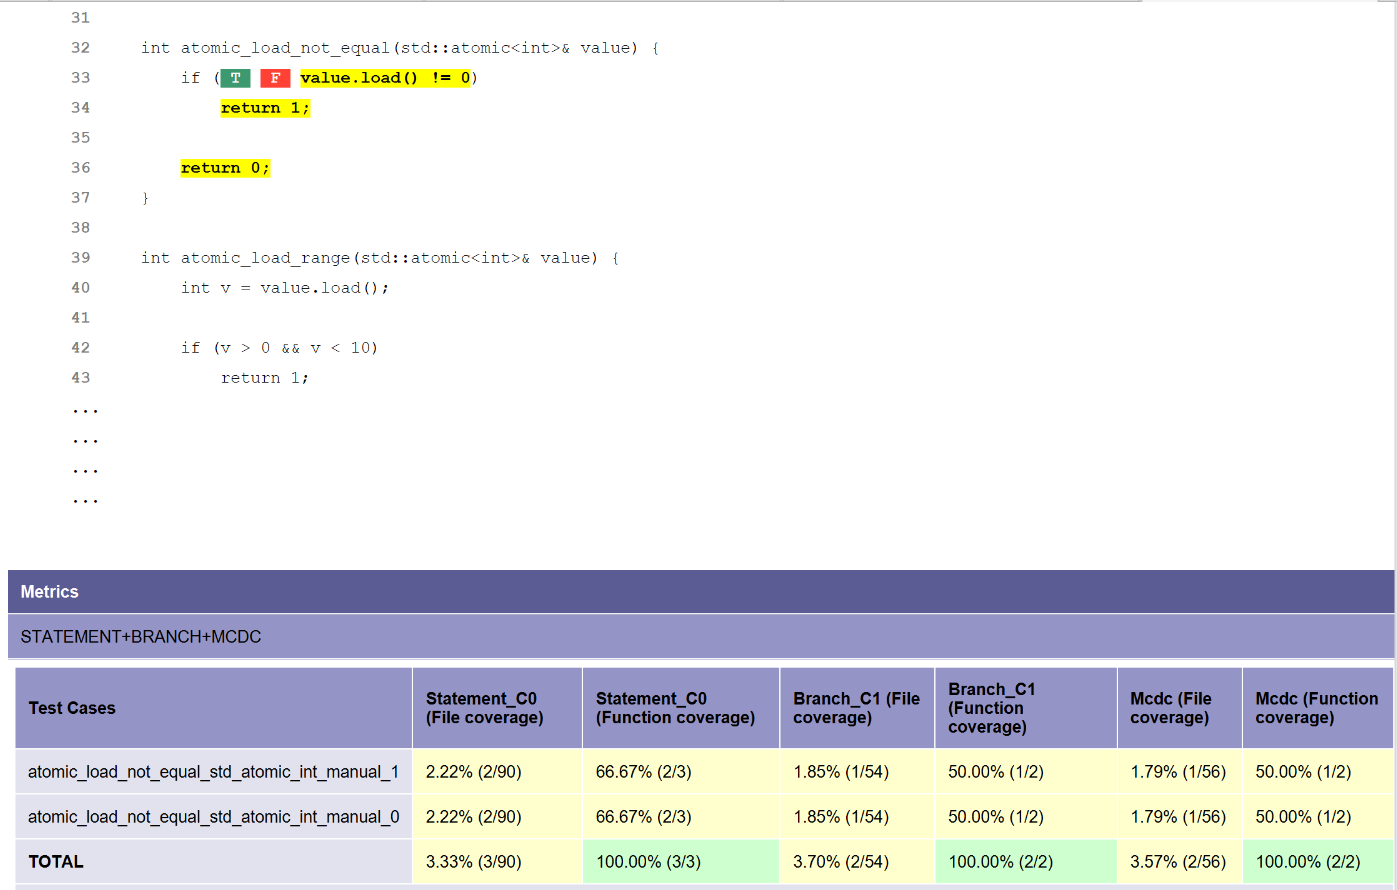
\includegraphics[width=0.9\textwidth]{images/atomic_execution.png}
\caption[Kết quả thực thi và độ phủ mã nguồn]{Kết quả thực thi và độ phủ mã nguồn của một hàm sử dụng \texttt{std::atomic}}
\label{fig:atomic_coverage}
\end{figure}


Đối với quá trình sinh test driver, hệ thống tạo thành công các câu lệnh khởi tạo sử dụng \texttt{store()} và xử lý việc sao chép dữ liệu nguyên tử thông qua cặp thao tác \texttt{load()}--\texttt{store()}. Các test driver được sinh ra đều có thể biên dịch và thực thi thành công trên các chương trình thực nghiệm.

Kết quả độ phủ mã nguồn cho thấy các nhánh điều kiện phụ thuộc vào giá trị của đối tượng \texttt{std::atomic} có thể được kích hoạt thông qua dữ liệu kiểm thử do người dùng cấu hình. Điều này chứng minh rằng cơ chế \texttt{AtomicDataNode} và các cải tiến trong bộ sinh test driver đã giúp AKAUTAUTO mở rộng phạm vi hỗ trợ đối với các chương trình sử dụng đối tượng nguyên tử.



% =====================================================================
%  Kết luận (chương không đánh số)
%  Nội dung: content/5.conclusion.tex
% =====================================================================
\chapter*{Kết luận}\label{Conclusion}
\addcontentsline{toc}{chapter}{Kết luận}

% chktex-file 13
% chktex-file 36
Báo cáo đã hoàn thành mục tiêu nghiên cứu và triển khai cơ chế hỗ trợ đối tượng \texttt{std::atomic} trong công cụ kiểm thử đơn vị tự động AKAUTAUTO. Thông qua quá trình khảo sát và phân tích kiến trúc hệ thống, nghiên cứu đã chỉ ra các hạn chế của phiên bản hiện tại khi xử lý biến nguyên tử, đặc biệt tại các giai đoạn nhận diện kiểu dữ liệu, biểu diễn dữ liệu kiểm thử và sinh mã kiểm thử.

Để khắc phục những hạn chế này, nghiên cứu đã đề xuất và cài đặt lớp \texttt{AtomicDataNode} nhằm biểu diễn đối tượng \texttt{std::atomic} trong cây dữ liệu kiểm thử. Bên cạnh đó, cơ chế sinh test driver cũng được mở rộng để hỗ trợ khởi tạo và xử lý dữ liệu nguyên tử thông qua các thao tác \texttt{load()} và \texttt{store()}, thay vì sử dụng phép gán trực tiếp như đối với các kiểu dữ liệu thông thường. Giải pháp được tích hợp vào kiến trúc hiện có của AKAUTAUTO mà không làm thay đổi các thành phần cốt lõi của hệ thống.

Kết quả thực nghiệm trên bộ chương trình gồm 25 hàm sử dụng \texttt{std::atomic} dưới nhiều hình thức khác nhau cho thấy hệ thống có thể nhận diện thành công các đối tượng nguyên tử, xây dựng chính xác \texttt{AtomicDataNode}, sinh mã kiểm thử hợp lệ và thực thi thành công các ca kiểm thử tương ứng. Các trường hợp thực nghiệm bao gồm tham số truyền tham chiếu, con trỏ, bí danh kiểu dữ liệu, đối tượng nguyên tử trong \texttt{struct}/\texttt{class}, các thao tác nguyên tử phổ biến như \texttt{load()}, \texttt{store()}, \texttt{exchange()}, \texttt{fetch\_*} và \texttt{compare\_exchange()}, cũng như các kịch bản liên quan đến cơ chế stub. Những kết quả này cho thấy giải pháp đề xuất đã mở rộng đáng kể phạm vi hỗ trợ của AKAUTAUTO đối với các chương trình C++ có sử dụng đối tượng nguyên tử.

Trong tương lai, nghiên cứu có thể được mở rộng theo nhiều hướng khác nhau. Thứ nhất, hệ thống có thể tiếp tục hỗ trợ đầy đủ hơn các thao tác của thư viện \texttt{std::atomic}, bao gồm các hàm nguyên tử nâng cao và các kiểu dữ liệu nguyên tử phức tạp hơn. Thứ hai, cơ chế sinh dữ liệu kiểm thử tự động có thể được tích hợp với bộ giải ràng buộc nhằm tự động tìm kiếm các giá trị đầu vào giúp kích hoạt những nhánh điều kiện phụ thuộc vào trạng thái của đối tượng nguyên tử. Cuối cùng, việc hỗ trợ các kịch bản đa luồng và phân tích tương tác đồng thời giữa nhiều đối tượng \texttt{atomic} là một hướng phát triển tiềm năng, góp phần nâng cao khả năng kiểm thử của AKAUTAUTO đối với các hệ thống phần mềm hiện đại.



\chapter*{Tài liệu tham khảo}
\addcontentsline{toc}{chapter}{Tài liệu tham khảo}
\printbibliography[keyword={vietnam}, heading=subbibliography, title={Tiếng Việt}, resetnumbers=true]
\printbibliography[notkeyword={vietnam}, heading=subbibliography, title=Tiếng Anh]

\end{document}
